\section{Bedienungsanleitung}
\vspace{0.5cm}
Voraussetzung für die Inbetriebnahme des Tools \glqq ShellBag Analyzer\grqq{} ist die Installation von Microsoft .NET Framework 4.8 \footnote{Download unter \url{https://www.chip.de/downloads/Microsoft-.NET-Framework-4.8_54812855.html}, zuletzt verfügbar am 15.06.2020}. Dies ist notwendig, um Anwendungen auszuführen, welche mit dem .NET Framework entwickelt wurden \cite{nett}. Mit dem Windows Update vom 10. Mai 2019 wird das .NET Framework 4.8 bereits mitgeliefert \cite{update}. Das Tool wird als ZIP-Datei zur Verfügung gestellt und muss zuvor entpackt werden. Anschließend kann die Datei \glqq ShellBag.GUI.exe\grqq{} ausgeführt werden. \\
\\
Falls ein Computer mehrere Nutzer enthält, so ist zunächst die SID des zu untersuchenden Benutzerkontos zu bestimmen. Bei der Analyse des aktuell angemeldeten Benutzers kann dessen SID mit dem Befehl \glqq \texttt{whoami /user}\grqq{} in der Eingabeaufforderung bestimmt werden. Dies ist notwendig, um den richtigen Benutzer im Tool oben links auszuwählen. Nach der Auswahl der jeweiligen SID erscheint der korrespondierende Benutzername sowie im unteren Bereich die Anzahl der ShellBags und die Ladezeit, die benötigt wurde, um die Informationen aus der Registry zu laden und auszuwerten. Nun kann im linken Bereich der Baum für die ShellBags der NTUSER.dat und  USRCLASS.dat aufgeklappt und ein Shell Item ausgewählt werden. Durch Klicken auf ein solches Item erscheinen im rechten Bereich die Art des Shell Items sowie die dazugehörigen Informationen. Diese werden tabellarisch aufgelistet. \\
\\
Um die Exportfunktion der ShellBags anzuwenden, ist in der obigen Menüleiste \glqq Datei - Exportieren - Textdatei (.txt)\grqq{} zu wählen. Die ShellBag-Informationen werden anschließend in Textdateien, getrennt voneinander für die NTUSER.dat und USRCLASS.dat, in dem Verzeichnis abgelegt, in dem sich die ausführbare Datei befindet. Diese Dateien können im Anschluss mit einem Editor geöffnet und eingesehen werden. \\
\\
Die Beendigung des Tools erfolgt entweder über die Menüleiste \glqq Datei - Beenden\grqq{} oder über das Kreuz-Symbol rechts oben. In beiden Fällen ist die Beendigung mit der Auswahl des Buttons \glqq Ja\grqq{} zu bestätigen. \\
\\
Die hier aufgeführten Informationen lassen sich ebenfalls im \glqq ShellBag Analyzer\grqq{} unter dem Menüpunkt \glqq Über\grqq{} einsehen. \\
\\
Die nachfolgende Abbildung \ref{img:analyzer} zeigt einen Ausschnitt des \glqq ShellBag Analyzers\grqq{}.

\begin{figure}[H]
	\centering
	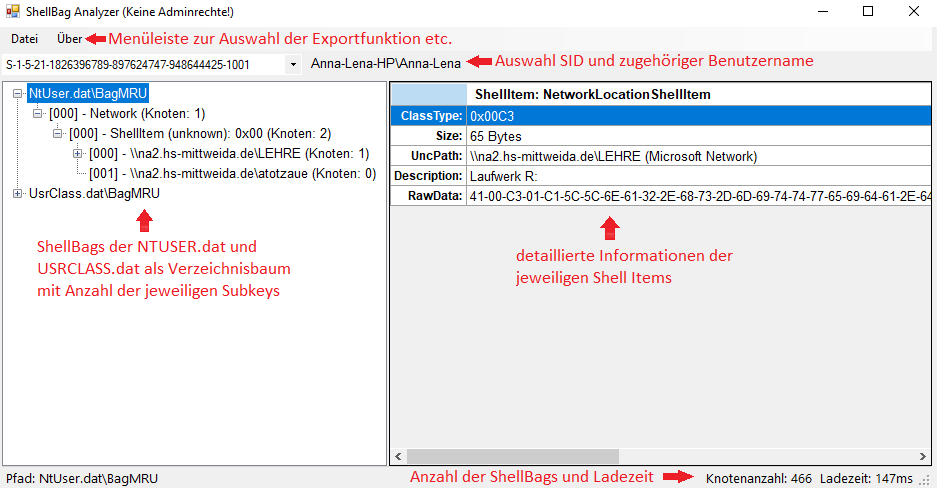
\includegraphics[width=1\textwidth]{part/analyzer.png}
	\caption{Ausschnitt des \glqq ShellBag Analyzers\grqq{}} 
	\label{img:analyzer}
\end{figure}
